\documentclass[12pt, a4paper]{article}
\usepackage[utf8]{inputenc}
\usepackage[portuguese]{babel}
\usepackage{titlesec}
\usepackage{titling}
\usepackage{indentfirst}
\usepackage{graphicx}
\graphicspath{{./images/} {/home/victor/Pictures/latex/}}
\usepackage{wrapfig}
\usepackage{fancyhdr}
\usepackage{colortbl}
\usepackage{color}
\usepackage{framed}
\usepackage{enumitem}
\usepackage{amsmath}
\usepackage{lastpage}
\usepackage[hyphens]{url}
\usepackage{hyperref}
\usepackage[brazilian,hyperpageref]{backref}
\usepackage[num,overcite,abnt-emphasize=bf]{abntex2cite}
%%\usepackage[alf,abnt-emphasize=bf]{abntex2cite}
%%\citebrackets()
\citebrackets[]

\hypersetup{
	colorlinks=true,
	linkcolor=black,
	filecolor=magenta,      
	urlcolor=blue,
	citecolor=blue,
}

% ---
% Configurações do pacote backref
% Usado sem a opção hyperpageref de backref
\renewcommand{\backrefpagesname}{Citado na(s) página(s):~}
% Texto padrão antes do número das páginas
\renewcommand{\backref}{}
% Define os textos da citação
\renewcommand*{\backrefalt}[4]{
  \ifcase #1 %
    Nenhuma citação no texto.%
    \or
    Citado na página #2.%
  \else
    Citado nas páginas #2.%
\fi}%
% ---

%% Definindo o Autor e o título
\newcommand{\prof}{Antonio M. M. Hachisuca}
%\newcommand{\materia}{}

\author{Victor Emanuel Almeida \and Marco Aurélio G. Pedroso}
\title{Manual}
\date{\today}

%% zera a pagina
\fancyfoot[C]{}
%% linhas no inicio e fim da página
\renewcommand{\headrulewidth}{0.7pt}
\renewcommand{\footrulewidth}{0.5pt}

%% Definindo espaçamento
%\titlespacing{\section}{0pt}{*2}{*1.1}
%%\titlespacing{\subsection}{}{}{}

%%Definindo formato de títulos
%%\titleformat{comando}[formato, ex:wrap]{mudar fontes}{antes do separador}{separador}{depois do separador}[no fim do comando]
%\titleformat{\section}
%{\large\tex}
%{\thesection}
%{.2cm}
%{}[\titlerule]

\begin{document}
\begin{titlepage}
	\centering
	\thispagestyle{fancy}

	\begin{minipage}{0.4\textwidth}
		\begin{flushleft}
			\includegraphics[scale=0.6]{logo_unioeste.jpg}\\[1.0 cm]
		\end{flushleft}
	\end{minipage}
	\begin{minipage}{0.5\textwidth}
		\begin{flushright}\large
			\textsc{\LARGE\textbf{UNIOESTE}}\\
			\vspace{1cm}
			Universidade Estadual\\do Oeste do Paraná
		\end{flushright}
	\end{minipage}
	%\rule{\textwidth}{.5pt}\\[2.0 cm]
	\vspace*{4.5 cm}

	{\huge\bfseries\thetitle}\\
	\rule{\linewidth}{0.2 mm}\\[1.5 cm]
	
	\vspace{2cm}
	\begin{minipage}[t]{0.4\textwidth}
		\begin{flushleft}\large
			\emph{Orientador:}\\
			\prof\\
		\end{flushleft}
	\end{minipage}
	\begin{minipage}[t]{0.5\textwidth}

		\begin{flushright}\large
			\emph{Alunos:}\\
			\theauthor
		\end{flushright}

	\end{minipage}\\[2 cm]
	
	\vfill\thedate
	\end{titlepage}

	\pagestyle{fancy}
	%\fancyfoot[L]{Aluno(s):~\theauthor}
	%\fancyfoot[R]{Prof:~\prof}
	\fancyfoot[L]{}
	\fancyfoot[R]{página~\thepage~de~\pageref{LastPage}}
	\fancyhead[L]{}
	\fancyhead[R]{}

	\tableofcontents
	\listoffigures
	\clearpage

	\section{Introdução}\label{Introdução}
	\subsection{Pré-requisitos}\label{Pré-requisitos}
	\begin{itemize}
		\item Placa de Rede 1 Gb.
		\item Uma quantidade ``$X$'' de painéis Led.
		\item Uma quantidade ``$X+1$'' de cabos de rede.
		\item Um computador com Windows.
	\end{itemize}

	\section{Instalação do software}\label{Instalação do software}
	Para instalar o software segue-se os seguintes passos:
	\begin{enumerate}
		\item Entrar no site da Nova Star na aba downloads\cite{siteDownload}
		\item Acessar a aba software.
		\begin{figure}[!htb]
			\centering
			
\includegraphics[width=\textwidth]{Download.png}
			\caption{\label{fig:Download}Aba de software dentro do site\cite{siteDownload}}
		\end{figure}
		\item Fazer o download do instalador do software NovaLCT.
		\begin{figure}[!htb]
			\centering
			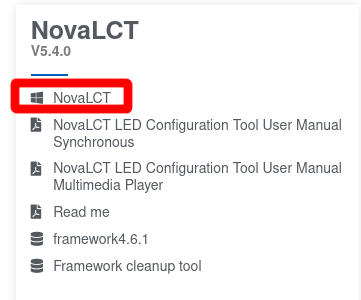
\includegraphics[scale=.9]{NOVALCT_INSTALL.png}
			\caption{\label{fig:NOVALCT_INSTALL}Baixando o executável do NovaLCT}
		\end{figure}
	\end{enumerate}

	\section{Conexão dos painéis}\label{Conexão dos painéis}

	\section{Configurando a rede}\label{Configurando a rede}

	\section{Configurando o software}\label{Configurando o software}
% ----------------------------------------------------------
% Referências bibliográficas
% ----------------------------------------------------------
\cleardoublepage
\bibliography{ref}

\end{document}
